% --------------------------------------------------------------------------------

\begin{exercise}

Verifizieren Sie den Stoke'schen Integralsatz für das Vektorfeld

\begin{align*}
    \mathbf F(x, y, z)
    =
    (1 - x y, x z, x + z)^t
\end{align*}

und das hyperbolische Paraboloid $z = x^2 - y^2$, $x^2 + y^2 < 1$.

\begin{align*}
    \Int[\gamma]
    {
        \mathbf F(t) \mathbf t
    }{t}
    & =
    \Int[0][2 \pi]
    {
        -
        \sin s + \cos s \sin^2 s
        +
        \cos^2 s (\cos^2 s - \sin^2 s)
        -
        2 (\cos s + \cos{2 s}) \sin{2 s}
    }{s} \\
    & =
    \Int[0][2 \pi]
    {
        \cos^2 s (1 - 2 \sin^2 s)
    }{s}
    =
    \pi
    -
    \Int[0][2 \pi]
    {
        \frac{1}{4}
        \sin^2{2 s}
    }{s}
    =
    \pi - \frac{\pi}{2}
    =
    \frac{\pi}{2}.
\end{align*}

\end{exercise}

% --------------------------------------------------------------------------------

\begin{solution}

\phantom{}

\includegraphicsboxed{Ana3/Ana3 - Satz 5.4.2 (Integralsatz von Stokes im R^3).png}

Sei $\Omega$ das hyperbolische Paraboloid.
Wir wollen das hyperbolische Paraboloid parametrisieren.
Das wurde netterweise in Beispiel 4.3.3 bereits gemacht.

\begin{tcolorbox}[standard jigsaw, opacityback = 0]
    \begin{center}
        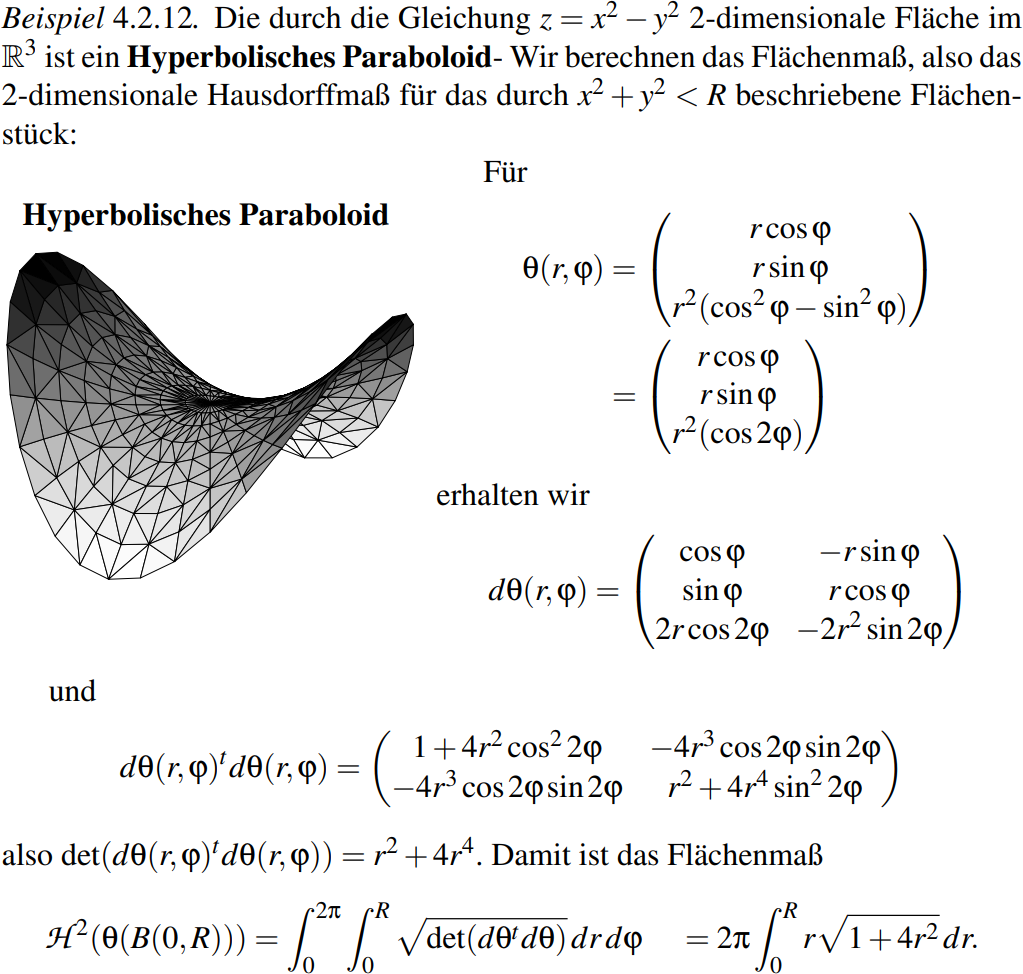
\includegraphics[width = 0.75 \textwidth]{Ana3/Ana3 - Beispiel 4.2.12.1.png}        
    \end{center}
    \hspace{1.85cm}
    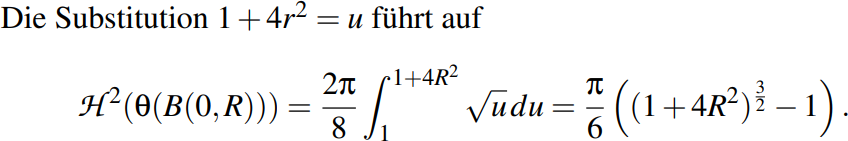
\includegraphics[width = 0.6  \textwidth]{Ana3/Ana3 - Beispiel 4.2.12.2.png}
\end{tcolorbox}

\begin{enumerate}[label = \arabic*.]

    \item Teil (\blockquote{lhs}):
    
    \begin{align*}
        \rot \mathbf F(x, y, z)
        =
        \begin{pmatrix}
            \derivative[][\mathbf F_3]{y}
            -
            \derivative[][\mathbf F_2]{z} \\
            \derivative[][\mathbf F_1]{z}
            -
            \derivative[][\mathbf F_3]{x} \\
            \derivative[][\mathbf F_2]{x}
            -
            \derivative[][\mathbf F_1]{y}
        \end{pmatrix}
        (x, y, z)
        =
        \begin{pmatrix}
            -x \\ -1 \\ z + x
        \end{pmatrix}
    \end{align*}

    Wir bestimmen das Normalvektorfeld.
    Dazu betrachten wir
    
    \begin{align*}
        N(x, y, z) := z - x^2 - y^2,
        \quad
        \text{mit}
        \quad
        \nabla N(x, y, z)
        =
        \begin{pmatrix}
            -2 x \\ 2 y \\ 1
        \end{pmatrix}.
    \end{align*}
    
    Das Normalvektorfeld lautet daher
    
    \begin{align*}
        \mathbf n:
            \Omega \to \R^3,
            (x, y, z)
            \mapsto
            \frac
            {
                \nabla N(x, y, z)
            }{
                |\nabla N(x, y, z)|
            }
            =
            \frac{1}{\sqrt{4 (x^2 + y^2) + 1}}
            \begin{pmatrix}
                -2 x \\ 2 y \\ 1
            \end{pmatrix}.
    \end{align*}

    Wir wollen Satz 4.2.15 anwenden.
    Daher berechnen wir noch

    \begin{align*}
        \vbraces
        {
            \derivative[][\theta]{r}
            \times
            \derivative[][\theta]{\varphi}
        }(x, y, z)
        & =
        \vbraces
        {
            \begin{pmatrix}
                \cos \varphi \\
                \sin \varphi \\
                2 r \cos{2 \varphi}
            \end{pmatrix}
            \times
            \begin{pmatrix}
                -r \sin \varphi \\
                 r \cos \varphi \\
                -2 r^2 \sin{2 \varphi}
            \end{pmatrix}
        } \\
        & =
        \vbraces
        {
            \begin{pmatrix}
                - \sin \varphi 2 r^2 \sin{2 \varphi} - 2 r \cos{2 \varphi} r \cos \varphi  \\
                -(r \sin \varphi 2 r \cos{2 \varphi} - \cos \varphi 2 r^2 \sin{2 \varphi}) \\
                \cos \varphi r \cos \varphi + r \sin \varphi \sin \varphi
            \end{pmatrix}
        } \\
        & =
        \vbraces
        {
            \begin{pmatrix}
                -2 r^2 (\sin \varphi \sin{2 \varphi} + \cos \varphi \cos{2 \varphi}) \\
                -2 r^2 (\sin \varphi \cos{2 \varphi} - \cos \varphi \sin{2 \varphi}) \\
                r (\cos^2 \varphi + \sin^2 \varphi)
            \end{pmatrix}
        } \\
        & =
        r
        \vbraces
        {
            \begin{pmatrix}
                -2 r \cos \varphi \\
                 2 r \sin \varphi \\
                 1
            \end{pmatrix}
        } \\
        & =
        r
        \sqrt{(-2 r \cos \varphi)^2 + (2 r \sin \varphi)^2 + 1^2} \\
        & =
        r
        \sqrt{ 4 r^2 (\cos^2 \varphi + \sin^2 \varphi) + 1} \\
        & =
        r
        \sqrt{4 r^2 + 1}.
    \end{align*}

    Wir verwenden Satz 4.2.15 und berechnen zu guter Letzt

    \begin{align*}
        &
        \Int[\Omega]
        {
            \rot \mathbf F \cdot \mathbf n
        }{
            \mathcal H^2
        } \\
        & =
        \Int[\theta(D)]
        {
            \frac{1}{\sqrt{4 (x^2 + y^2) + 1}}
            (2 x^2 - 2 y + z + x)
        }{
            \mathcal H^2(x, y, z)
        } \\
        & =
        \int_D
            \frac{1}{\sqrt{4 ((r \cos \varphi)^2 + (r \sin \varphi)^2) + 1}}
            (2 (r \cos \varphi)^2 - 2 (r \sin \varphi) + r^2 \cos{2 \varphi} + (r \cos \varphi)) \\
        & \quad \quad \quad
            \vbraces
            {
                \derivative[][\theta]{r}
                \times
                \derivative[][\theta]{\varphi}
            }(r, \varphi)
            ~\mathrm d(r, \varphi) \\
        & =
        \Int[0][1]
        {
            \Int[0][2 \pi]
            {
                \frac{1}{\sqrt{4 r^2 (\cos^2 \varphi + \sin^2 \varphi) + 1}}
                (2 r^2 \cos^2 \varphi - 2 r \sin \varphi + r^2 \cos{2 \varphi} + r \cos \varphi)
                r
                \sqrt{4 r^2 + 1}
            }{\varphi}
        }{r} \\
        & =
        \Int[0][1]
        {
            \Int[0][2 \pi]
            {
                2 r^3 \cos^2 \varphi
            }{\varphi}
        }{r}
        -
        \Int[0][1]
        {
            \Int[0][2 \pi]
            {
                2 r^2 \sin \varphi
            }{\varphi}
        }{r}
        +
        \Int[0][1]
        {
            \Int[0][2 \pi]
            {
                r^3 \cos{2 \varphi}
            }{\varphi}
        }{r} \\
        & \quad
        +
        \Int[0][1]
        {
            \Int[0][2 \pi]
            {
                r^2 \cos \varphi
            }{\varphi}
        }{r} \\
        & =
        2
        \underbrace
        {
            \Int[0][2 \pi]
            {
                \cos^2 \varphi
            }{\varphi}
        }_\pi
        \underbrace
        {
            \Int[0][1]
            {
                r^3
            }{r}
        }_\frac{1}{4}
        -
        2
        \underbrace
        {
            \Int[0][2 \pi]
            {
                \sin \varphi
            }{\varphi}
        }_0
        \underbrace
        {
            \Int[0][1]
            {
                r^2
            }{r}
        }_\frac{1}{3}
        +
        \underbrace
        {
            \Int[0][2 \pi]
            {
                \cos{2 \varphi}
            }{\varphi}
        }_0
        \underbrace
        {
            \Int[0][1]
            {
                r^3
            }{r}
        }_\frac{1}{4} \\
        & \quad
        +
        \underbrace
        {
            \Int[0][2 \pi]
            {
                \cos \varphi
            }{\varphi}
        }_0
        \underbrace
        {
            \Int[0][1]
            {
                r^2
            }{r}
        }_\frac{1}{3} \\
        & =
        \frac{\pi}{2}.
    \end{align*}
    
    \item Teil (\blockquote{rhs}):

    Wir verwenden $\gamma := \theta(1, \cdot)$ und berechnen

    \begin{align*}
        &
        \Int[\partial \Omega]
        {
            \mathbf F^t \cdot \mathbf t
        }{
            \mathcal H^1
        } \\
        & =
        \Int[\gamma]
        {
            \mathbf F
        }{(x, y, z)} \\
        & =
        \Int[0][2 \pi]
        {
            \mathbf F(\gamma(s)) \gamma^\prime(s)
        }{s} \\
        & =
        \Int[0][2 \pi]
        {
            (1 - \cos s \sin s)  (-\sin s)
            +
            (\cos s \cos{2 s})   (\cos s)
            +
            (\cos s + \cos{2 s}) (-2 \sin{2 s})
        }{s} \\
        & =
        \Int[0][2 \pi]
        {
            -\sin s + \cos s \sin^2 s + \cos^2 s \cos{2 s} - 2 \cos s \sin{2 s} - 2 \cos {2 s} \sin{2 s}
        }{s} \\
        & =
        -
        \underbrace
        {
            \Int[0][2 \pi]
            {
                \sin s
            }{s}
        }_0
        +
        \underbrace
        {
            \Int[0][2 \pi]
            {
                \cos s \sin^2 s
            }{s}
        }_0
        +
        \underbrace
        {
            \Int[0][2 \pi]
            {
                \cos^2 s \cos{2 s}
            }{s}
        }_\frac{\pi}{2}
        -
        2
        \underbrace
        {
            \Int[0][2 \pi]
            {
                \cos s \sin{2 s}
            }{s}
        }_0 \\
        & \quad
        -
        2
        \underbrace
        {
            \Int[0][2 \pi]
            {
                \cos{2 s} \sin{2 s}
            }{s}
        }_0 \\
        & =
        \frac{\pi}{2}.
    \end{align*}

\end{enumerate}

\end{solution}

% --------------------------------------------------------------------------------
